\section{Components}

\subsection{Mechanical components}
\subsubsection{Central Body}

Used to host the flywheel, a motor and a bearing.
\begin{figure}[H]
    \centering
    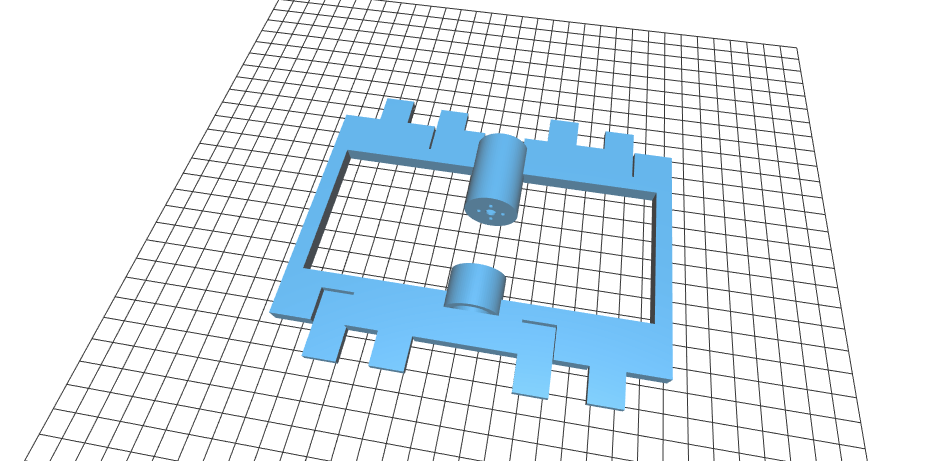
\includegraphics[width=10cm]{img/components/central_body.png}
    \caption{3D Model of the central body.}
    \label{fig:Mass plot}
\end{figure}
\subsubsection{Lateral Body}
\begin{figure}[H]
    \centering
    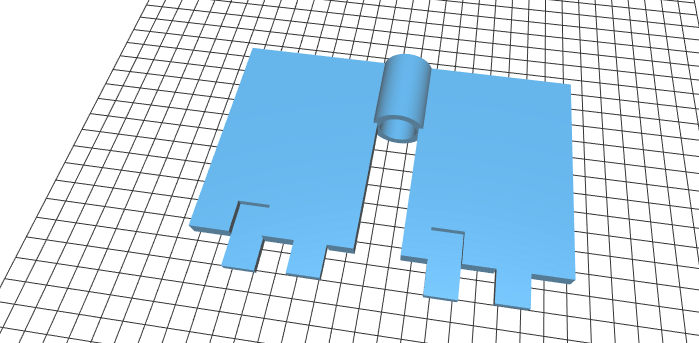
\includegraphics[width=10cm]{img/components/lateral_body.png}
    \caption{3D Model of lateral body.}
    \label{fig:Mass plot}
\end{figure}
\subsubsection{Wheels}
\begin{figure}[H]
    \centering
    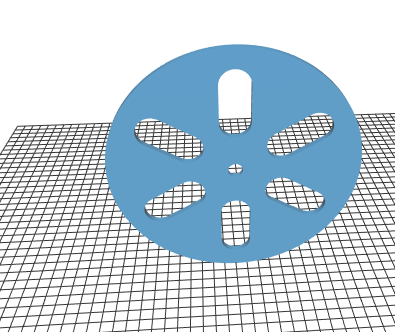
\includegraphics[width=10cm]{img/components/wheel.png}
    \caption{3D Model of a wheel.}
    \label{fig:Mass plot}
\end{figure}
\subsubsection{Flywheel}
\subsubsection{Bearings}
\subsection{Electronic components}
\subsubsection{Raspberry Pi}
The Raspberry Pi is a small single-board computer. We are using Raspberry Pi 3 Model B. It has GPIO pins.
\begin{figure}[H]
    \centering
    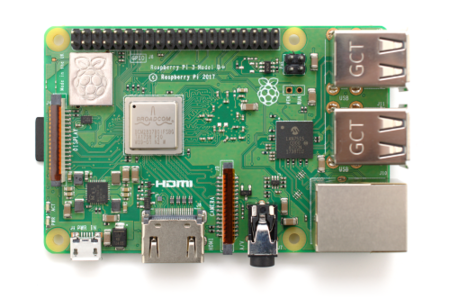
\includegraphics[width=10cm]{img/components/raspberry_pi.png}
    \caption{Raspberry Pi picture}
    \label{fig:Mass plot}
\end{figure}
\begin{center}
    \begin{tabular}{ |c|c| }
        \hline
        Weight          & 42 g      \\
        \hline
        Price per unit  & 35 euros \\
        \hline
        Number of units & 1        \\
        \hline
    \end{tabular}
\end{center}
\subsubsection{Batteries}
Provide power to our motors and to the Raspberry Pi.
\subsubsection{Breadboard}
A breadboard is a construction base for prototyping of electronics.
\subsubsection{DC Motor}
A DC motor is a class of rotary electrical machines that converts
direct current electrical energy into mechanical energy. The most common
types rely on the forces produced by magnetic fields.
\begin{center}
    \begin{tabular}{ |c|c| }
        \hline
        Operating voltage       & between 3 V and 9 V \\
        \hline
        Free-run speed at 6 V   & 176 RPM             \\
        \hline
        Free-run current at 6 V & 80 mA               \\
        \hline
        Stall current at 6V     & 900 mA              \\
        \hline
        Stall current at 6V     & 5 kg·cm             \\
        \hline
        Gear ratio              & 1:35                \\
        \hline
        Reductor size           & 21 mm               \\
        \hline
        Weight                  & 85 g                \\
        \hline
        Price per unit          & 10 euros            \\
        \hline
        Number of units         & 3                   \\
        \hline
    \end{tabular}
\end{center}

\subsubsection{H Bridge}
An H bridge is an electronic circuit that switches the polarity of a
voltage applied to a load. These circuits are often used in robotics
and other applications to allow DC motors to run forwards or backwards.
\subsubsection{Rotatory Encoder}
A rotary encoder, also called a shaft encoder, is an electro-mechanical device that converts the
angular position or motion of a shaft or axle to analog or digital output signals.
\subsubsection{Accelerometer}
An accelerometer is a device that measures proper acceleration. Proper acceleration, being the
acceleration (or rate of change of velocity) of a body in its own instantaneous rest frame, is not the same as coordinate acceleration, being the acceleration in a fixed coordinate system.
For example, an accelerometer at rest on the surface of the Earth will measure an acceleration due
to Earth's gravity, straight upwards (by definition) of g ≈ 9.81 m/s2.
